\documentclass[11pt]{article}
\usepackage[margin=1in]{geometry}
\usepackage{graphicx}
\usepackage{booktabs}
\usepackage[hidelinks]{hyperref}
\title{RhythmBot: Project Progress Report}
\author{Anna Deng \and Yifan Kang}
\date{November 23, 2026}
\begin{document}
\maketitle
\section*{Current progress}
We have built single-arm and dual-arm Drake environments for taps, holds, and
continuous slides. We compare classical planning, Code as Policy (CAP), and
behavior cloning (BC). CAP generates executable Python controllers with Codex;
``initial,'' ``feedback 1,'' and ``feedback 2'' denote successive programs revised
using training feedback. BC learns either a multilayer perceptron (MLP) or a
diffusion action model from demonstrations. Our two-arm setup uses one stylus
per arm, a minimal Project SEKAI-inspired screen, and simulated camera RGB
with robot occlusion. We have completed the original 330-run dual-arm study,
then added 220 matched color/shape versus neural-vision runs and 66 sequential
live BC runs. We use 11 held-out charts and three training seeds per BC model.
The frozen neural detector now receives geometrically rectified camera pixels,
including its predicted remaining slide path; it receives no chart state.
\begin{figure}[ht]
\centering
\begin{minipage}[b]{.49\linewidth}
\centering
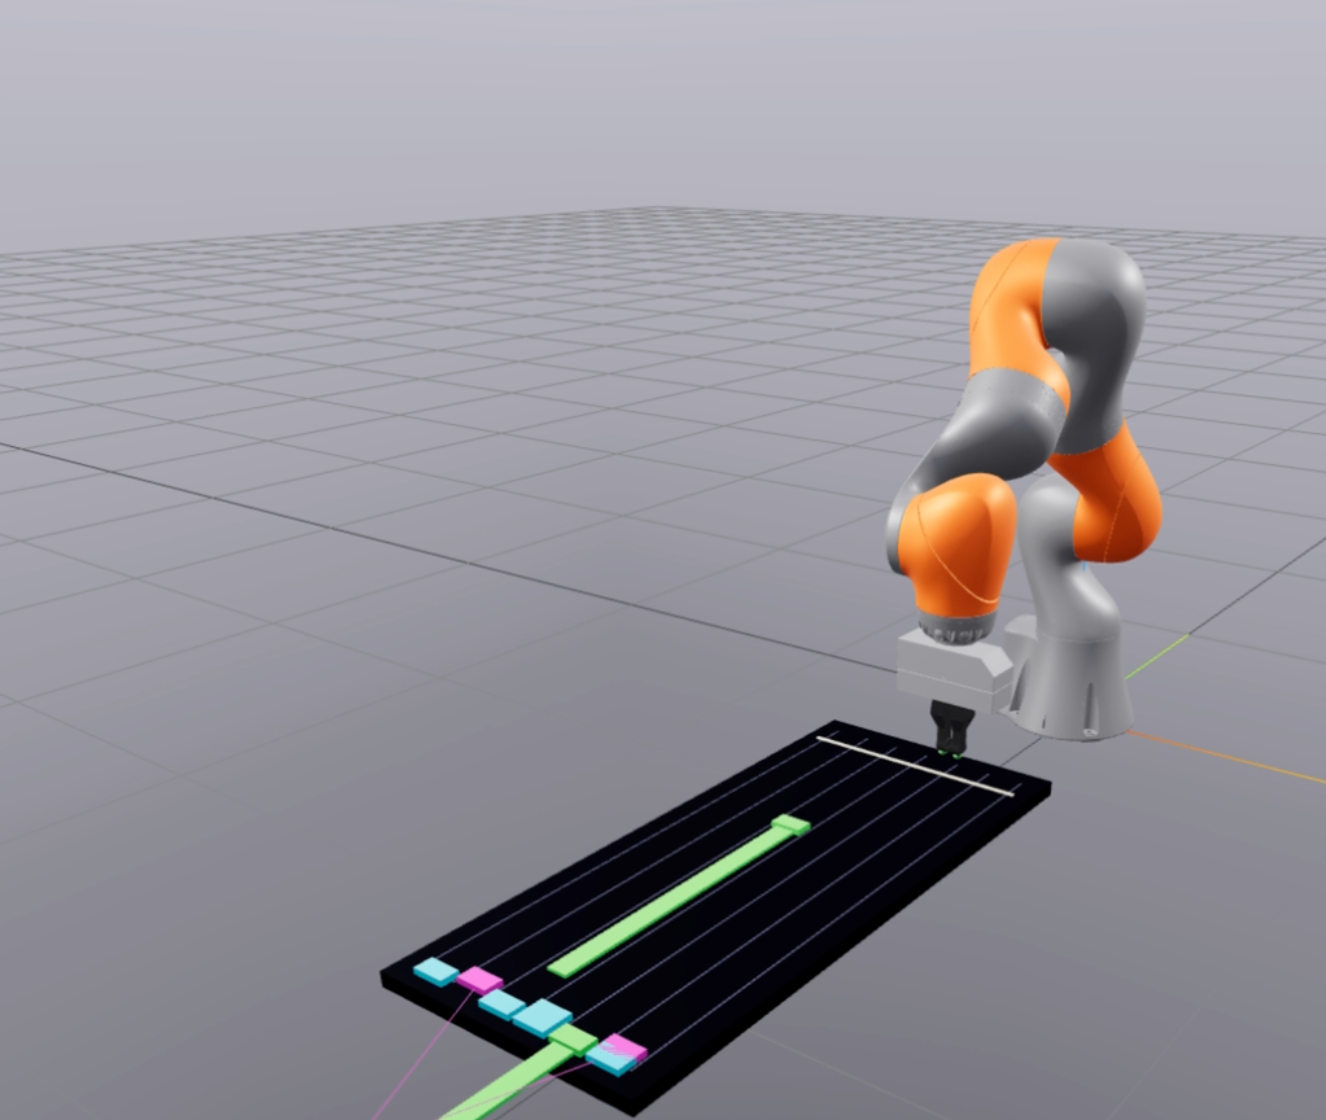
\includegraphics[width=\linewidth,height=2.7in,keepaspectratio]{assets/single-arm.png}\\[6pt]
(a) Single-arm environment
\end{minipage}\hfill
\begin{minipage}[b]{.49\linewidth}
\centering
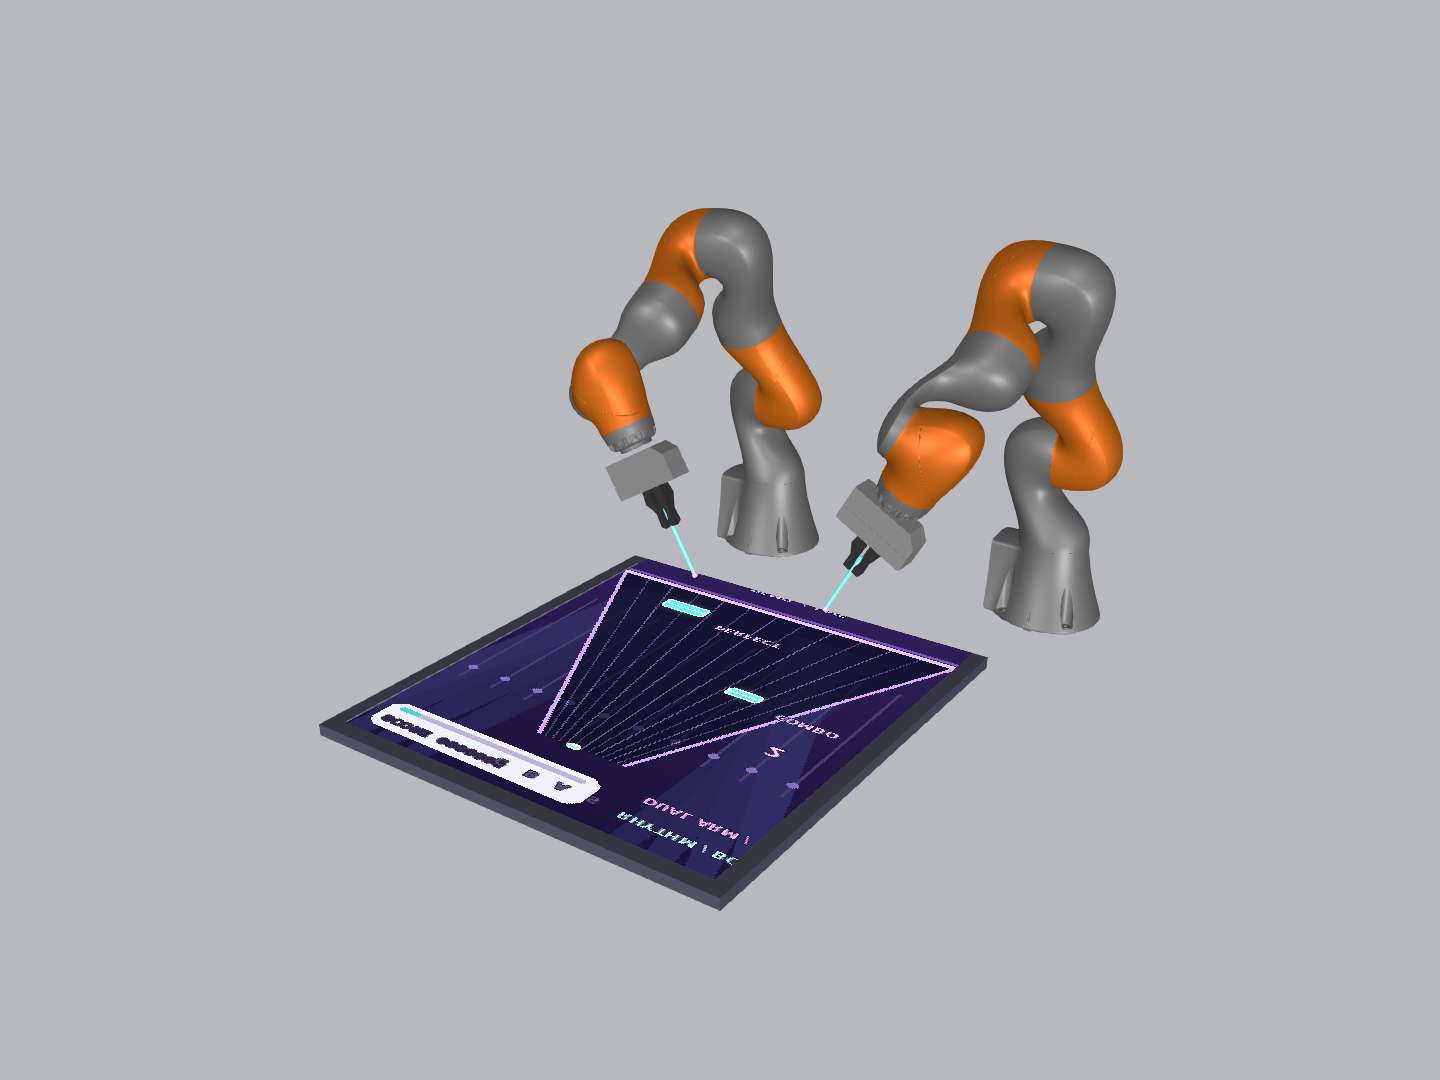
\includegraphics[width=\linewidth,height=2.7in,keepaspectratio]{assets/camera.png}\\[6pt]
(b) Dual-arm environment
\end{minipage}
\caption{Our Drake environments with native Meshcat robot rendering. The dual-arm
screen has only lanes, notes, and the judgment line. These are observer views;
control uses a separate fixed simulated RGB camera.}
\end{figure}
\newpage
\section*{Results and next steps}
We completed all registered runs without execution errors, while retaining strict
slide continuity and tail judgments. On the matched 960$\times$720 camera test,
classical completion is 89.2\% with color/shape vision and 84.5\%
with the frozen neural detector; MLP BC reaches 37.3\% and 55.3\%,
and diffusion BC 56.0\% and 55.6\%, respectively. The neural model
was trained on a different display: this is zero-shot transfer, not retraining
on the new screen. In separate 640$\times$480 live tests with color/shape vision,
Meshcat publishing, and the original ten-step diffusion sampler, MLP and
diffusion use 1.002 and 1.262 wall seconds per simulated second.
Only 17 of 66 runs meet our maximum-lag limit of one 30\,Hz frame.
These measurements exclude startup and browser display latency. Our next steps
are adapting neural perception using training-only camera data and reducing
controller latency; completed experiments do not imply reliable real-time play.
\begin{figure}[ht]
\centering
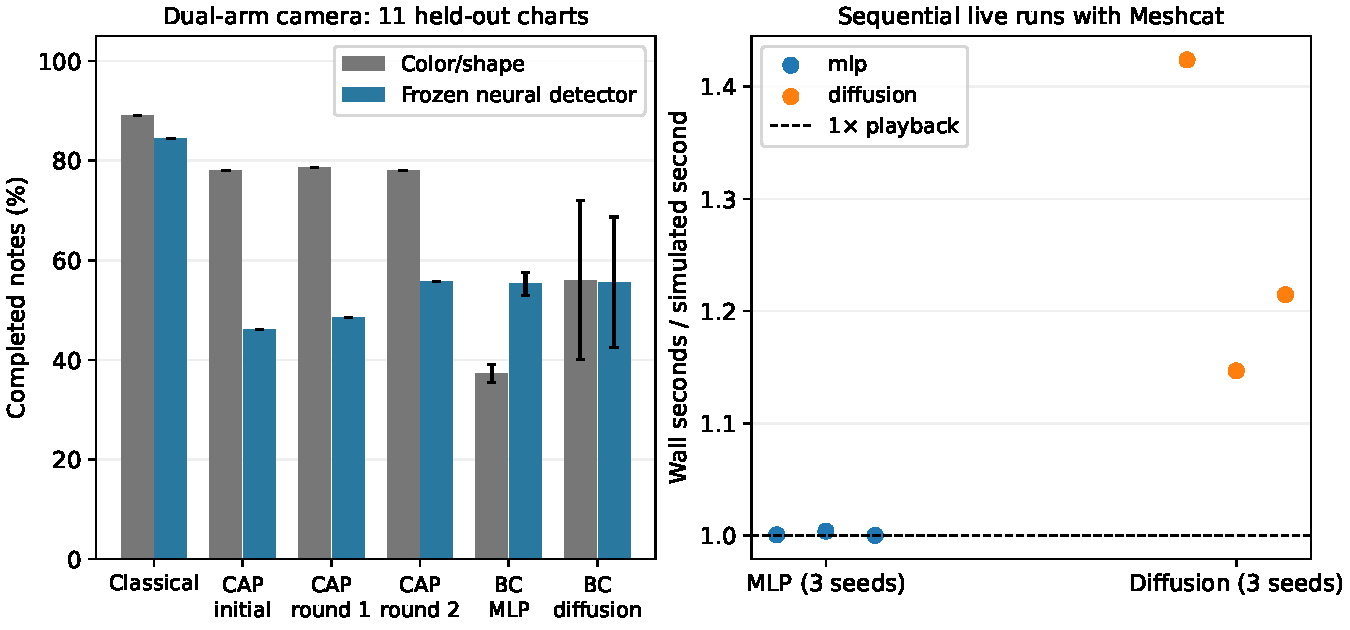
\includegraphics[width=\linewidth]{assets/remaining-results.pdf}
\caption{Dual-arm results on the same 11 held-out charts. BC error bars show sample
standard deviation across three training seeds. CAP rounds 1 and 2 are
training-feedback revisions of one initial program. Live points aggregate 11 charts per seed. Accuracy uses full note
completion, including sustain contact and tails.}
\end{figure}
\begin{table}[ht]
\centering
\begin{tabular}{lcc}
\toprule
Live controller & Wall / simulation time & One-frame lag passes\\
\midrule
MLP BC & 1.002 & 17 / 33\\
Diffusion BC & 1.262 & 0 / 33\\
\bottomrule
\end{tabular}
\caption{Sequential Apple M5 measurements with two Drake arms and Meshcat.
A near-1$\times$ average does not guarantee that individual frames meet deadlines.}
\end{table}
\end{document}
